\pdfminorversion=7%
\documentclass[aspectratio=169,mathserif,notheorems]{beamer}%
%
\xdef\bookbaseDir{../../bookbase}%
\xdef\sharedDir{../../shared}%
\RequirePackage{\bookbaseDir/styles/slides}%
\RequirePackage{\sharedDir/styles/styles}%
%
\gdef\searchSpace{\ensuremath{\mathbb{X}}}%
\gdef\sespel{\ensuremath{x}}%
\gdef\opti#1{\ensuremath{#1^{\star}}}%
%
%% Print an algorithm box around something.
\protected\gdef\algobox#1#2{\resizebox{#1\paperwidth}{!}{%
\bgroup%
\fboxsep=0pt%
\fboxrule=2pt%
\mbox{\fcolorbox{white}{white}{\bgroup%
\fboxsep=2pt%
\fboxrule=2pt%
\mbox{\fcolorbox{hfuu-red!80}{hfuu-orange!60}{%
\mbox{#2}%
}}\egroup%
}}%
\egroup}}%
%
\title{Frequency Fitness Assignment}%
%
\begin{document}%
\startPresentation%
%
\section{Introduction}%
%
\begin{frame}[t]%
\frametitle{Introduction to Optimization}%
\begin{itemize}%
\item Optimization means finding superlatives.%
\item<2-> Find the \alert{fastest} way to get from Hefei to Beijing.%
\item<3-> Find the \alert{shortest} route through $n$~cities.%
\item<4-> Set the pricing for these apples such that we can get the \alert{largest} revenue when selling them.%
\item<5-> Place all these chips on a circuit board so that they occupy the \alert{smallest} area while we can still properly connect and cool them.%
\item<6-> Find the \alert{cheapest} way to transport these goods from Hefei to Wellington.%
\item<7-> Design an airplane wing with the \alert{least} aerodynamic drag.%
\item<8-> Find a strategy to manage the power of the nodes in this sensor network so that full coverage is guaranteed for the \alert{longest} possible duration.%
\item<9-> And so on.%
\end{itemize}%
\locateGraphic{1}{width=0.85\paperwidth}{\sharedDir/graphics/optimization_superlatives/optimization_superlatives}{0.075}{0.2}%
\locateGraphic{2-}{width=0.35\paperwidth}{\sharedDir/graphics/optimization_superlatives/optimization_superlatives}{0.63}{0.01}%
\end{frame}%
%
\begin{frame}[t]%
\frametitle{Views on Optimization}%
\begin{itemize}%
\only<-1>{\item There are two ways to look at optimization.}%
\only<-2>{\item<2-> The economic view.}%
\item<3-> The mathematical view.%
\end{itemize}%
\locateGraphic{2}{width=0.75\paperwidth}{\sharedDir/graphics/optimization_views/optimization_views_1}{0.125}{0.3}%
\locateGraphic{3}{width=0.75\paperwidth}{\sharedDir/graphics/optimization_views/optimization_views_2}{0.125}{0.3}%
\end{frame}%
%
\begin{frame}%
\frametitle{Example: Traveling Salesperson Problem}%
\parbox{0.373\paperwidth}{%
\begin{itemize}%
%
\item In the \glsFull{TSP}\cite{ABCC2006TTSPACS,LLRKS1985TTSPAGTOCO,GP2002TTSPAIV,WCLTTCMY2014BOAAOSFFTTSP}, the goal is to find the shortest round-ttrip tour through a set of $n$~cities.%
%
\item<2-> The search space \searchSpace\ thus is the set of all possible round-trip tours through these $n$~cities, usually specified as permutations of the first $n$~natural numbers.%
%
\item<3-> The objective function~$f:\searchSpace\mapsto\realNumbers$, subject to minimization, is the length of the tour.%
%
\item<4-> The optimal solution~$\opti{\sespel}\in\searchSpace$ is the shortest possible tour.%
%
\end{itemize}%
}%
%
\locateGraphic{-3}{width=0.525\paperwidth}{\sharedDir/graphics/tsp_china/tsp_china}{0.44}{0.15}%
\locateGraphic{4-}{width=0.525\paperwidth}{\sharedDir/graphics/tsp_china/tsp_china_solution}{0.44}{0.15}%
%
\end{frame}%
%
\begin{frame}%
\frametitle{Example: Maximum Satisfiability Problem}%
\parbox{0.42\paperwidth}{%
\begin{itemize}%
%
\item The goal of the \glsFull{MaxSAT}\cite{HS2004SLSFAA,C1971TCOTPP} problem is to find a setting of \textcolor<2>{red}{$n$~variables} that makes a Boolean formula~$F$ become True. %
The variables appear directly or \textcolor<3>{violet}{negated} in \textcolor<4>{blue}{$m$~OR\nobreakdashes-clauses}, whose results flow into \textcolor<5>{green!40!black}{one AND\nobreakdashes-clause}.%
%
\item<6-> \searchSpace\ is the set of all possible bit strings of length~$n$.%
%
\item<7-> The objective function~$f:\searchSpace\mapsto\realNumbers$ is the number of unsatisfied OR\nobreakdashes-clauses.%
%
\item<8-> The optimum~$\opti{\sespel}\in\searchSpace$ has $f(\opti{\sespel})=0$, i.e., all clauses satisfied, i.e., $F(\opti{\sespel})=\textnormal{True}$.%
%
\end{itemize}%
}%
%
\locateGraphic{-1,6-}{width=0.5\paperwidth}{\sharedDir/graphics/sat/sat_plain}{0.47}{0.3}%
\locateGraphic{2}{width=0.5\paperwidth}{\sharedDir/graphics/sat/sat_variables}{0.47}{0.3}%
\locateGraphic{3}{width=0.5\paperwidth}{\sharedDir/graphics/sat/sat_negated}{0.47}{0.3}%
\locateGraphic{4}{width=0.5\paperwidth}{\sharedDir/graphics/sat/sat_clauses}{0.47}{0.3}%
\locateGraphic{5}{width=0.5\paperwidth}{\sharedDir/graphics/sat/sat_and}{0.47}{0.3}%
%
\end{frame}%
%
\begin{frame}[t]%
\frametitle{Example: Bin Packing Problem}%
\begin{itemize}%
\item The goal of the Bin Packing Problem is to pack $n$~objects, each having a specific size, into as few bins~(also of a given size) as possible.%
\item<2-> The \searchSpace\ comprises all possible packing orders of the $n$~objects.%
\item<3-> The objective function~$f$ is the number of bins needed by a given packing order.%
\item<4-> The optimum~$\opti{\sespel}$ is the packing order requiring the fewest bins.%
\end{itemize}%
\locateGraphic{}{width=0.85\paperwidth}{\sharedDir/graphics/bin_packing/bin_packing}{0.075}{0.5}%
\end{frame}%
%
\begin{frame}[t]%
\frametitle{Optimization is Hard}%
\begin{itemize}%
%
\item Finding the globally optimal solution~\opti{\sespel} from the set of all possible solutions~\searchSpace\ is often an \npHard\ problem.%
%
\item<2-> Currently, there is no algorithm that can \alert{guarantee} to find the optimal solution of \alert{every instance} of a given \npHard\ problem in a runtime that is not longer than polynomial in the size of the problem~(i.e., existing algorithms may need exponential runtime in the \alert{worst case}).%
%
\item<3-> In other words, if we want to guarantee to find the best possible solution~\opti{\sespel} for all possible instances of a problem, we often cannot really be much faster than testing all possible candidate solutions~$\sespel\in\searchSpace$ in the \alert{worst case}.%
%
\end{itemize}%
\end{frame}%
%
\section{Metaheuristic Optimization}%
%
\begin{frame}%
\frametitle{Metaheuristic Optimization}%
\parbox{0.42\paperwidth}{%
\begin{itemize}%
%
\item Metaheuristics follow the Trial-and-Error idea of iterative improvement.%
\item<2-> They drop the guarantee to find the optimal solution.%
\item<3-> They try to find good solution within a feasible runtime.%
\item<4-> They start with random solutions.%
\item<5-> And then roughly follow this cycle.%
%
\end{itemize}%
}%
%
\locateGraphic{5}{width=0.5\paperwidth}{\sharedDir/graphics/metaheuristic_cycle/metaheuristic_cycle_01}{0.47}{0.3}%
%
\locateGraphic{6}{width=0.5\paperwidth}{\sharedDir/graphics/metaheuristic_cycle/metaheuristic_cycle_02}{0.47}{0.3}%
%
\locateGraphic{7}{width=0.5\paperwidth}{\sharedDir/graphics/metaheuristic_cycle/metaheuristic_cycle_03}{0.47}{0.3}%
%
\locateGraphic{8}{width=0.5\paperwidth}{\sharedDir/graphics/metaheuristic_cycle/metaheuristic_cycle_04}{0.47}{0.3}%
%
\locateGraphic{9}{width=0.5\paperwidth}{\sharedDir/graphics/metaheuristic_cycle/metaheuristic_cycle_05}{0.47}{0.3}%
%
\locateGraphic{10}{width=0.5\paperwidth}{\sharedDir/graphics/metaheuristic_cycle/metaheuristic_cycle_06}{0.47}{0.3}%
%
\locateGraphic{11}{width=0.5\paperwidth}{\sharedDir/graphics/metaheuristic_cycle/metaheuristic_cycle_07}{0.47}{0.3}%
%
\end{frame}%
%
\begin{frame}[t]%
\frametitle{The $(1+1)$~EA and RLS}%
\begin{itemize}%
\item Local search with $|S_i|=|N_i|=1$ is the simplest realization of the metaheuristic idea.%
\item<2-> \GlsFull{algoRLS} and the \glsFull{algoEAopo} work according the same pattern~(and differ only in their unary search operator~$\mathop{move}$)\cite{DJW2002OTAOTOPOEA,CPD2018TAMPARAOEA}.%
\item<8-> They accept the new solution if it is better or equally good compared to the current solution.%
\end{itemize}%
%
%
\locate{2}{%
\algobox{0.75}{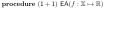
\includegraphics[width=0.75\paperwidth]{\sharedDir/graphics/metaheuristic_algorithms/opoea/opoea_1}}%
}{0.125}{0.445}%
%
\locate{3}{%
\algobox{0.75}{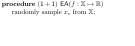
\includegraphics[width=0.75\paperwidth]{\sharedDir/graphics/metaheuristic_algorithms/opoea/opoea_2}}%
}{0.125}{0.445}%
%
\locate{4}{%
\algobox{0.75}{\includegraphics[width=0.75\paperwidth]{\sharedDir/graphics/metaheuristic_algorithms/opoea/opoea_3}}%
}{0.125}{0.445}%
%
\locate{5}{%
\algobox{0.75}{\includegraphics[width=0.75\paperwidth]{\sharedDir/graphics/metaheuristic_algorithms/opoea/opoea_4}}%
}{0.125}{0.445}%
%
\locate{6}{%
\algobox{0.75}{\includegraphics[width=0.75\paperwidth]{\sharedDir/graphics/metaheuristic_algorithms/opoea/opoea_5}}%
}{0.125}{0.445}%
%
\locate{7}{%
\algobox{0.75}{\includegraphics[width=0.75\paperwidth]{\sharedDir/graphics/metaheuristic_algorithms/opoea/opoea_6}}%
}{0.125}{0.445}%
%
\locate{8}{%
\algobox{0.75}{\includegraphics[width=0.75\paperwidth]{\sharedDir/graphics/metaheuristic_algorithms/opoea/opoea_7}}%
}{0.125}{0.445}%
%
\locate{9}{%
\algobox{0.75}{\includegraphics[width=0.75\paperwidth]{\sharedDir/graphics/metaheuristic_algorithms/opoea/opoea_8}}%
}{0.125}{0.445}%
%
\locate{10}{%
\algobox{0.75}{\includegraphics[width=0.75\paperwidth]{\sharedDir/graphics/metaheuristic_algorithms/opoea/opoea_9}}%
}{0.125}{0.445}%
%
\locate{11-}{%
\algobox{0.75}{\includegraphics[width=0.75\paperwidth]{\sharedDir/graphics/metaheuristic_algorithms/opoea/opoea}}%
}{0.125}{0.445}%
%
\end{frame}%
%
\begin{frame}%
\frametitle{Simulated Annealing}%
\parbox{0.41\paperwidth}{%
\begin{itemize}%
\item \glsFull{algoSA}\cite{KGV1983OBSA,C1985TATTTSPAESA,DPSW1982MCTICO,P1970AMCMFTASOCTOCOP} is a local search that accepts also worsening moves, but with a probability that decreases over time AND with the difference in solution quality.%
\item<7-> The probability is regulated by temperature schedule with parameter\only<10->{s}~$T_0$\only<10->{ and~$\epsilon$}.%
\item<11-> It also remembers best-so-far solution~$x_B$ and its objective value~$y_B$, because it could get lost.%
\end{itemize}%
}%
%
%
\locate{2}{%
\algobox{0.5}{\includegraphics[width=0.5\paperwidth]{\sharedDir/graphics/metaheuristic_algorithms/sa/sa_01}}%
}{0.44}{0.24}%
%
\locate{3}{%
\algobox{0.5}{\includegraphics[width=0.5\paperwidth]{\sharedDir/graphics/metaheuristic_algorithms/sa/sa_02}}%
}{0.44}{0.24}%
%
\locate{4}{%
\algobox{0.4}{\includegraphics[width=0.4\paperwidth]{\sharedDir/graphics/metaheuristic_algorithms/sa/sa_02}}%
}{0.44}{0.07}%
%
\locate{4}{%
\resizebox{0.5\paperwidth}{!}{\bgroup%
\fboxsep=2pt%
\fboxrule=2pt%
\fcolorbox{black}{white}{%
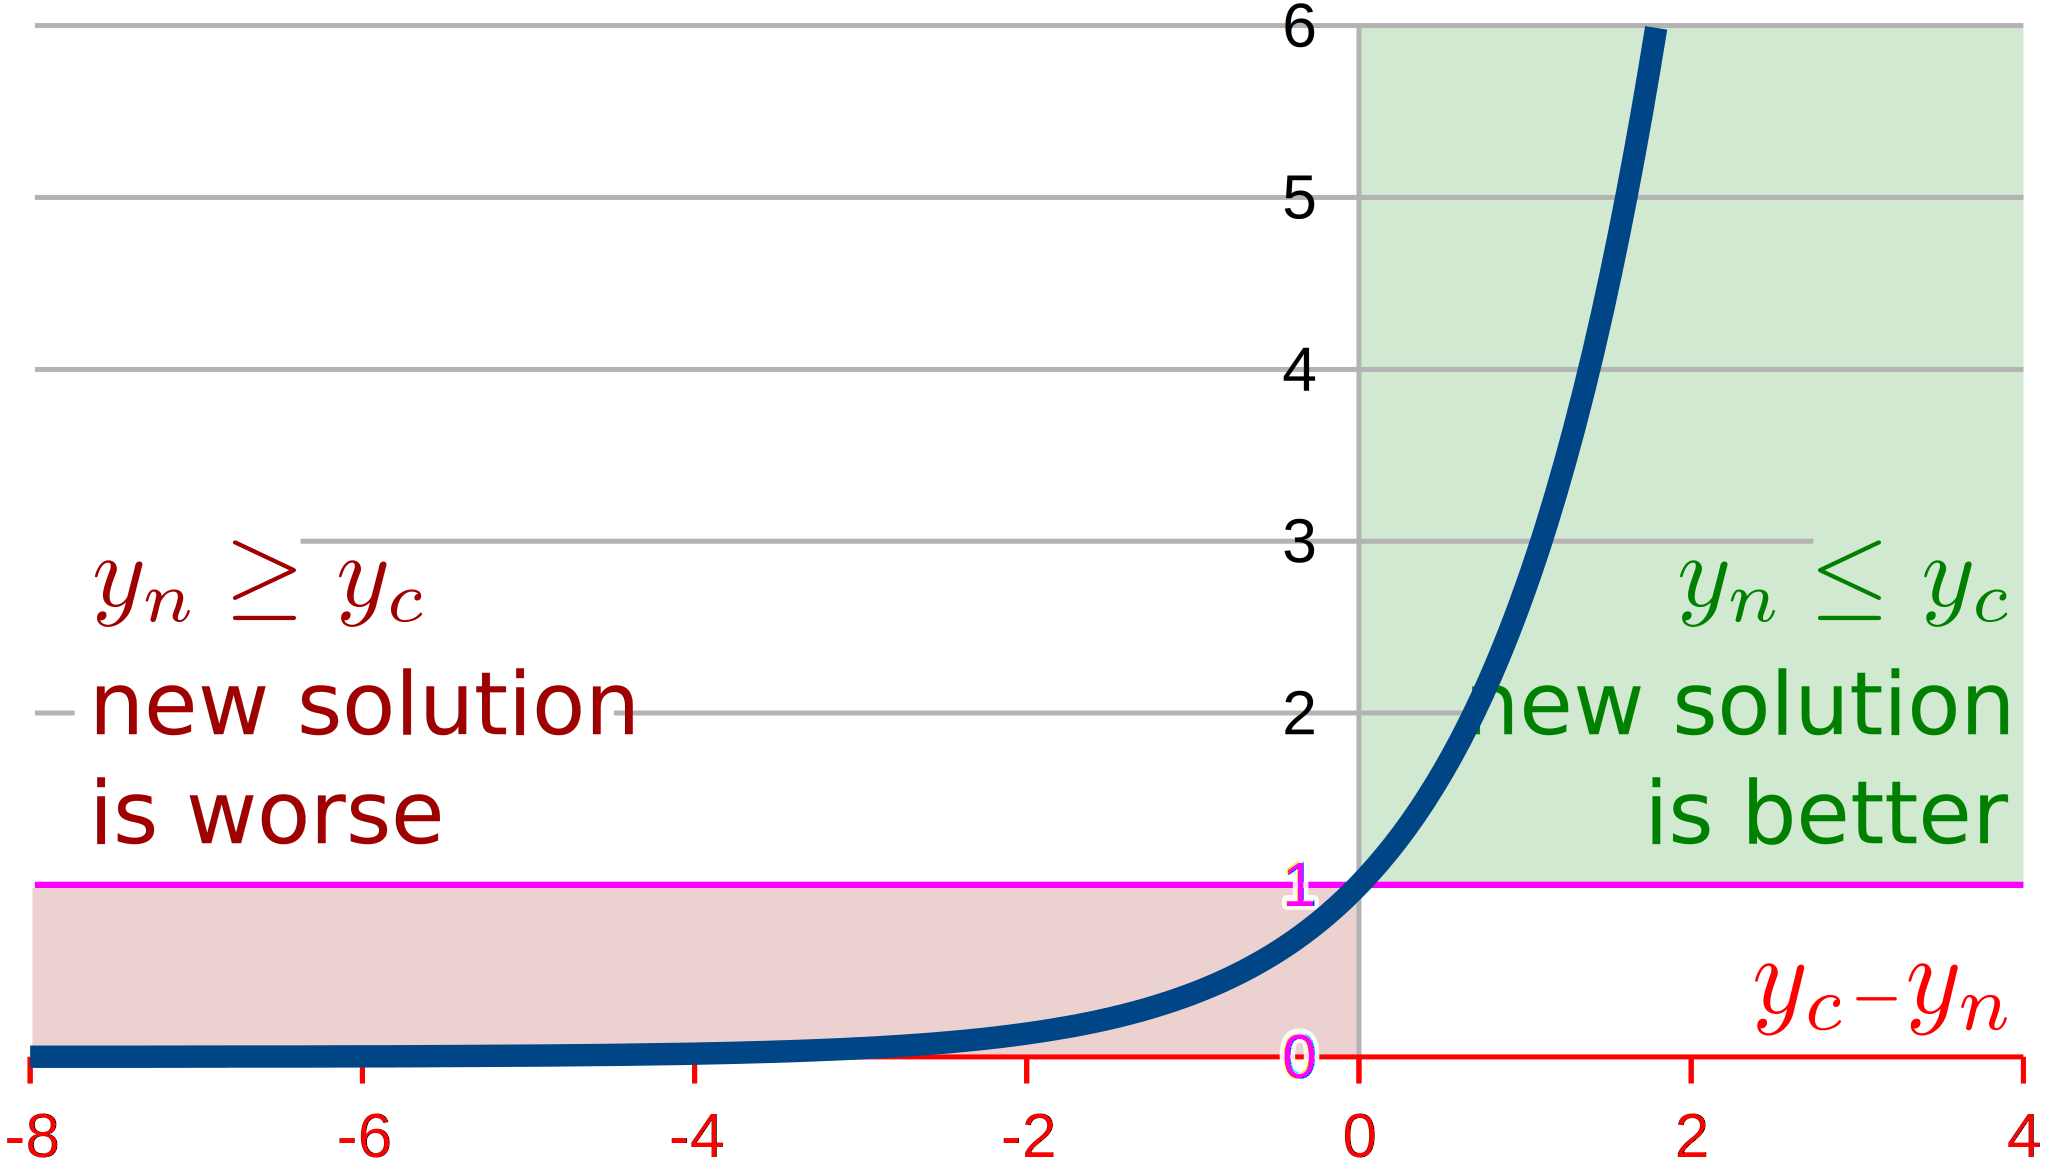
\includegraphics[width=0.5\paperwidth]{\sharedDir/graphics/metaheuristic_algorithms/sa/exp}%
}%
\egroup}%%
}{0.46}{0.41}%
%
\locate{5}{%
\algobox{0.5}{\includegraphics[width=0.5\paperwidth]{\sharedDir/graphics/metaheuristic_algorithms/sa/sa_03}}%
}{0.44}{0.24}%
%
\locate{6}{%
\algobox{0.5}{\includegraphics[width=0.5\paperwidth]{\sharedDir/graphics/metaheuristic_algorithms/sa/sa_04}}%
}{0.44}{0.24}%
%
\locate{7}{%
\algobox{0.5}{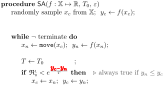
\includegraphics[width=0.5\paperwidth]{\sharedDir/graphics/metaheuristic_algorithms/sa/sa_05}}%
}{0.44}{0.24}%
%
\locate{8}{%
\algobox{0.5}{\includegraphics[width=0.5\paperwidth]{\sharedDir/graphics/metaheuristic_algorithms/sa/sa_06}}%
}{0.44}{0.24}%
%
\locate{9}{%
\algobox{0.5}{\includegraphics[width=0.5\paperwidth]{\sharedDir/graphics/metaheuristic_algorithms/sa/sa_07}}%
}{0.44}{0.24}%
%
\locate{10}{%
\algobox{0.5}{\includegraphics[width=0.5\paperwidth]{\sharedDir/graphics/metaheuristic_algorithms/sa/sa_08}}%
}{0.44}{0.24}%
%
\locate{11}{%
\algobox{0.5}{\includegraphics[width=0.5\paperwidth]{\sharedDir/graphics/metaheuristic_algorithms/sa/sa_09}}%
}{0.44}{0.24}%
%
\locate{12}{%
\algobox{0.5}{\includegraphics[width=0.5\paperwidth]{\sharedDir/graphics/metaheuristic_algorithms/sa/sa_10}}%
}{0.44}{0.24}%
%
\locate{13}{%
\algobox{0.5}{\includegraphics[width=0.5\paperwidth]{\sharedDir/graphics/metaheuristic_algorithms/sa/sa}}%
}{0.44}{0.24}%
%
\end{frame}%
%
\begin{frame}%
\frametitle{Standard Genetic Algorithm with Roulette Wheel Selection}%
\parbox{0.41\paperwidth}{%
\begin{itemize}%
\item The \glsFull{algoSGA} with Fitness Proportionate Selection~(Roulette Wheel) is for \textcolor{blue}{maximization}\cite{G1989GA,DJ2006ECAUA,W2009GOATAA,BFM1997HOEC,M1996GADSEP,M1998AITGA}.%
\item<2-> It uses a population of size~$ps$ as well as a unary\only<9->{ and binary} operator\only<9->{~(with crossover rate~$cr$)}.%
\end{itemize}%
}%
%
\locate{2}{%
\algobox{0.5}{\includegraphics[width=0.5\paperwidth]{\sharedDir/graphics/metaheuristic_algorithms/sga/sga_01}}%
}{0.44}{0.24}%
%
\locate{3}{%
\algobox{0.5}{\includegraphics[width=0.5\paperwidth]{\sharedDir/graphics/metaheuristic_algorithms/sga/sga_02}}%
}{0.44}{0.24}%
%
\locate{4}{%
\algobox{0.5}{\includegraphics[width=0.5\paperwidth]{\sharedDir/graphics/metaheuristic_algorithms/sga/sga_03}}%
}{0.44}{0.24}%
%
\locate{5}{%
\algobox{0.5}{\includegraphics[width=0.5\paperwidth]{\sharedDir/graphics/metaheuristic_algorithms/sga/sga_04}}%
}{0.44}{0.24}%
%
\locate{6}{%
\algobox{0.5}{\includegraphics[width=0.5\paperwidth]{\sharedDir/graphics/metaheuristic_algorithms/sga/sga_05}}%
}{0.44}{0.24}%
%
\locate{7}{%
\algobox{0.5}{\includegraphics[width=0.5\paperwidth]{\sharedDir/graphics/metaheuristic_algorithms/sga/sga_06}}%
}{0.44}{0.24}%
%
\locate{8}{%
\algobox{0.5}{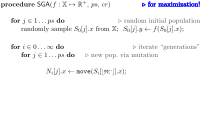
\includegraphics[width=0.5\paperwidth]{\sharedDir/graphics/metaheuristic_algorithms/sga/sga_07}}%
}{0.44}{0.24}%
%
\locate{9}{%
\algobox{0.5}{\includegraphics[width=0.5\paperwidth]{\sharedDir/graphics/metaheuristic_algorithms/sga/sga_08}}%
}{0.44}{0.24}%
%
\locate{10}{%
\algobox{0.5}{\includegraphics[width=0.5\paperwidth]{\sharedDir/graphics/metaheuristic_algorithms/sga/sga_09}}%
}{0.44}{0.24}%
%
\locate{11}{%
\algobox{0.5}{\includegraphics[width=0.5\paperwidth]{\sharedDir/graphics/metaheuristic_algorithms/sga/sga_10}}%
}{0.44}{0.24}%
%
\locate{12}{%
\algobox{0.5}{\includegraphics[width=0.5\paperwidth]{\sharedDir/graphics/metaheuristic_algorithms/sga/sga_11}}%
}{0.44}{0.24}%
%
\locate{13}{%
\algobox{0.5}{\includegraphics[width=0.5\paperwidth]{\sharedDir/graphics/metaheuristic_algorithms/sga/sga_12}}%
}{0.44}{0.24}%
%
\locate{14}{%
\algobox{0.5}{\includegraphics[width=0.5\paperwidth]{\sharedDir/graphics/metaheuristic_algorithms/sga/sga_13}}%
}{0.44}{0.24}%
%
\locate{15}{%
\algobox{0.5}{\includegraphics[width=0.5\paperwidth]{\sharedDir/graphics/metaheuristic_algorithms/sga/sga}}%
}{0.44}{0.24}%
%
\end{frame}%
%
\section{Advertisement}%
%
\begin{frame}[t]%
\frametitle{Programming with Python}%
We have a freely available course book on \citetitle{programmingWithPython} at \citeurl{programmingWithPython}, with focus on practical software development using the \python\ ecosystem of tools\cite{programmingWithPython}.%
%
\locateGraphic{}{width=0.63\paperwidth}{\sharedDir/graphics/advertisement/snippets/programmingWithPythonSnippet}{0.025}{0.3}%
\locateGraphic{}{width=0.27\paperwidth}{\sharedDir/graphics/advertisement/urlQr/programmingWithPythonCourseUrl}{0.675}{0.4}%
%
\end{frame}%
%
\begin{frame}[t]%
\frametitle{Databases}%
We have a freely available course book on \citetitle{databases} at \citeurl{databases}, with actual practical examples using a real \dbms\cite{databases}.%
%
\locateGraphic{}{width=0.63\paperwidth}{\sharedDir/graphics/advertisement/snippets/databasesSnippet}{0.025}{0.3}%
\locateGraphic{}{width=0.27\paperwidth}{\sharedDir/graphics/advertisement/urlQr/databasesCourseUrl}{0.675}{0.4}%
%
\end{frame}%
%
%
\endPresentation%
\end{document}%%
\endinput%
%
